\documentclass[11pt,a4paper]{article}
\usepackage[margin=2.4cm]{geometry}
\usepackage{amsmath,amssymb}
\usepackage{graphicx}
\usepackage{booktabs}
\usepackage{siunitx}
\usepackage[hidelinks]{hyperref}
\usepackage{microtype}

\newcommand{\TAWSS}{\mathrm{TAWSS}}
\newcommand{\OSI}{\mathrm{OSI}}
\newcommand{\RRT}{\mathrm{RRT}}
\newcommand{\eps}{\varepsilon}

\title{Cancellation, not accuracy: a first-order theory of residence-time
error in time-resolved hemodynamic surrogates, and why the error triple
$(\TAWSS,\OSI,\RRT)$ identifies the kind of error}

\author{Suvam Samanta\thanks{\texttt{suvam.samanta60@gmail.com}. Affiliation to be added.}}
\date{Draft, 19 September 2026}

\begin{document}
\maketitle

\begin{abstract}
Time-resolved deep-learning surrogates for wall shear stress (WSS) are
evaluated by a field error and by the cycle-averaged biomarkers $\TAWSS$,
$\OSI$ and $\RRT$. These three are not independent measures of accuracy:
they are algebraic functions of two time integrals of the same field,
coupled through the cancellation ratio
$R=|\int\boldsymbol\tau\,dt|/\int|\boldsymbol\tau|\,dt$. We give the
first-order response of $R$ to an arbitrary perturbation
$\mathbf d(t)$,
$\delta R/R=\hat{\mathbf s}\cdot\langle\mathbf d\rangle/(R\langle|\boldsymbol\tau|\rangle)
-\langle\hat{\boldsymbol\tau}\cdot\mathbf d\rangle/\langle|\boldsymbol\tau|\rangle$,
and evaluate it in closed form for the error types surrogates actually have.
(i)~For a \emph{window mismatch} --- integrating over the patient's period
when the surrogate's period differs and is unknown, the situation for an
autoregressive rollout --- the amplification is
$2\sqrt{m_-^2q_++m_+^2q_-}/[(m_++m_-)(m_+-m_-)]$ in terms of the first two
moments of the positive and negative parts of $\boldsymbol\tau$. Its exponent
in $X=1/R-1$ is $5/6$ at the onset of reversal, where the reversed lobe is
parabolic, and $1$ for broad reversal; the previously fitted $0.64$ is this
geometry combined with the growth of the field error itself with reversal.
A pure period change integrated over the surrogate's own period leaves all
three biomarkers exactly unchanged. (ii)~For a \emph{persistent spatial bias}
the exponent is $1$ with a larger prefactor, $(\delta R/R)/\eps=X+2f_-$ in
one dimension, so cancellation punishes bias about five times harder than
window mismatch at equal field error; the formula predicts the measured
per-face response on patient CFD to within $10\%$ in every reversing bin.
(iii)~Temporally white noise is suppressed by $1/\sqrt N$ in both terms.
$\RRT$ is exactly invariant to temporal smoothing. Consequences: on a
POD\,+\,LSTM surrogate rolled out at an unseen heart rate, a one-step RMSE of
$7\times10^{-2}$ hides a limit cycle running $1.4\%$ fast, recoverable from
the rollout alone without ground truth, yet re-timing repairs only a fifth of
the $\RRT$ error because the rest is beat shape; and the published error
triple of an independent per-snapshot graph surrogate (RHSIA:
$13.5/68.4/17.3\%$) falls in the spatial-bias band
($\OSI/\TAWSS=5.05$ against $1.2$ for window mismatch and $30$ for white
noise), which its authors confirm. The three numbers every surrogate paper
already reports therefore diagnose whether the remedy is re-timing,
smoothing, or a better model.
\end{abstract}

\section{Introduction}

Surrogates that predict the WSS vector over the cardiac cycle from a vascular
surface mesh are being proposed as a route to clinical use of CFD-derived
biomarkers~\cite{npj2026,jekenrico2025,rhsia2026,rygiel2025}. They are
graded by a relative $L_2$ error on the field and by the errors of the
cycle-averaged biomarkers $\TAWSS$, $\OSI$ and $\RRT$. Across these papers
$\OSI$ is reported as the hardest quantity, and the explanation offered is
that $\OSI$ ``is numerically sensitive'' or ``is small over most of the
surface''~\cite{rhsia2026,aaa2025}. The fragility of $\OSI$ to resolution,
inflow and noise has been noted for a decade in the CFD and 4D-flow
literature~\cite{sarrami2016,bergersen2017,mri2016}.

This note derives the sensitivity instead of observing it. The three
biomarkers are algebraic functions of two time integrals of the same field,
and their errors under a common perturbation are coupled through one
dimensionless number, the cancellation ratio $R$. Section~\ref{sec:theory}
gives the first-order response of $R$ to an arbitrary perturbation and
evaluates it in closed form for the three error types surrogates actually
have; the exponents that control $\RRT$ error come out of the geometry of the
reversed lobe of the waveform, not from a fit, and they differ by error type.
That difference is what makes the error triple diagnostic: the ratio
$\OSI/\TAWSS$ identifies which perturbation a model is suffering from. We
then test the predictions on two patient geometries, on a trained surrogate,
and on numbers published by an independent group.

The work was carried out for the UnivaXBio hackathon (Devpost, October 2026),
where the same analysis is packaged as an interactive ``unit test'' for
hemodynamic surrogates. The present note records the scientific content
separately so that it can be cited and checked.

\section{Definitions and first-order theory}
\label{sec:theory}

Let $\boldsymbol\tau(t)$ be the WSS vector at a wall face over one period
$T$, and write $\langle\cdot\rangle$ for the time mean over that period.
Define
\begin{equation}
M=\langle|\boldsymbol\tau|\rangle,\qquad
\mathbf S=\langle\boldsymbol\tau\rangle,\qquad
S=|\mathbf S|,\qquad
R=\frac{S}{M}\in[0,1],
\end{equation}
so that
\begin{equation}
\TAWSS=M,\qquad
\OSI=\frac{1-R}{2},\qquad
\RRT=\frac{1}{(1-2\,\OSI)\,\TAWSS}=\frac{1}{S}.
\end{equation}
$R$ is the fraction of the unsigned shear that survives the time integral;
$1-R$ is what cancels. $\RRT$ is the reciprocal of the \emph{net} shear
alone. Throughout, $X\equiv1/R-1=2\OSI/(1-2\OSI)$ is the cancellation
factor: cancelled shear divided by surviving shear.

\subsection{Response to an arbitrary perturbation}

Let the surrogate produce $\boldsymbol\tau+\mathbf d$ with
$|\mathbf d|\ll|\boldsymbol\tau|$. Then
$\delta M=\langle\hat{\boldsymbol\tau}\cdot\mathbf d\rangle$ with
$\hat{\boldsymbol\tau}=\boldsymbol\tau/|\boldsymbol\tau|$, and
$\delta S=\hat{\mathbf s}\cdot\langle\mathbf d\rangle$ with
$\hat{\mathbf s}=\mathbf S/S$, so
\begin{equation}
\boxed{\;\frac{\delta R}{R}
=\frac{\hat{\mathbf s}\cdot\langle\mathbf d\rangle}{R\,M}
-\frac{\langle\hat{\boldsymbol\tau}\cdot\mathbf d\rangle}{M}\;}
\label{eq:master}
\end{equation}
and, since $\delta\RRT/\RRT=-\delta S/S$ and
$\delta\TAWSS/\TAWSS=\delta M/M$,
\begin{equation}
\frac{\delta\RRT}{\RRT}=\frac{\delta\TAWSS}{\TAWSS}+\frac{\delta R}{R},
\qquad
\frac{\delta\OSI}{\OSI}=-\frac{R}{1-R}\,\frac{\delta R}{R}.
\label{eq:chain}
\end{equation}
The first term of \eqref{eq:master} carries the $1/R$: the perturbation's
\emph{time average} is divided by the surviving shear, which is small
wherever cancellation is strong. The second term has no such factor. Two
structural consequences are immediate. A perturbation with
$\langle\mathbf d\rangle=\mathbf 0$ leaves $S$, hence $\RRT$, unchanged
regardless of its size --- temporal smoothing is of this kind, and on the
sweep below the $\RRT$ error under a box filter is $7\times10^{-16}$. And a
pure time shift of a periodic signal changes none of the three biomarkers, so
the field error $\eps$ that appears in any of the formulas below must be
measured \emph{after} removing the best global time offset; the raw $L_2$
between a drifting rollout and the truth grows with accumulated lag and
overstates biomarker error badly (Section~\ref{sec:lstm}).

What remains is to evaluate \eqref{eq:master} for the perturbations that
surrogates actually produce. The three below have closed forms and,
importantly, different exponents in $X$.

\subsection{Window mismatch (a rollout with the wrong period)}
\label{sec:window}

A surrogate whose limit cycle runs a factor $1+\rho$ fast reproduces the
waveform exactly; nothing is wrong with it except the rate. If the biomarkers
are integrated over \emph{its own} period, all three are unchanged exactly,
because they are means over a full cycle of the same function. This point is
due to W.\ Ding (personal communication, 2026); it means a clock error is
harmless whenever the period is known, as it is for a model with a
prescribed inflow phase.

The error arises when the period is \emph{not} known and the biomarkers are
integrated over the patient's period $T$ instead. That window then covers
$1+\rho$ of the surrogate's cycles, and to first order the perturbation is
the extra slice $\mathbf d=\rho\,\boldsymbol\tau(\theta)$ at the phase
$\theta$ where the window closes. Substituting into \eqref{eq:master} and
taking the rms over $\theta$ --- the phase is arbitrary and unknown --- gives,
in one dimension, with $m_\pm=\langle\tau^\pm\rangle$ and
$q_\pm=\langle(\tau^\pm)^2\rangle$ the first two moments of the positive and
negative parts of $\tau$,
\begin{equation}
\frac{(\delta R/R)_{\rm rms}}{\rho}
=\frac{2\sqrt{m_-^2q_++m_+^2q_-}}{(m_++m_-)(m_+-m_-)}\;\equiv\;F,
\qquad
X=\frac{2m_-}{m_+-m_-}.
\label{eq:window}
\end{equation}
Equation~\eqref{eq:window} is exact in the waveform and contains no fitted
constant. Its exponent in $X$ follows from the geometry of the reversed lobe.

\paragraph{Onset of reversal: $p=5/6$.}
Let the waveform just dip below zero, by a depth $\delta$. For any smooth
$\tau$ the reversed lobe is locally parabolic, so its width scales as
$\sqrt\delta$ and
\begin{equation}
m_-\sim\delta^{3/2},\qquad q_-\sim\delta^{5/2},
\end{equation}
while $m_+$ and $q_+$ are $O(1)$. Then $X\sim\delta^{3/2}$ and the numerator
of \eqref{eq:window} is dominated by $m_-\sqrt{q_+}\sim\delta^{3/2}$ against
$m_+\sqrt{q_-}\sim\delta^{5/4}$, the latter winning as $\delta\to0$; hence
$F\sim\delta^{5/4}=X^{5/6}$. The exponent $5/6$ is universal for smooth
waveforms at the onset of reversal, independent of $\alpha$ and of the
waveform's detailed shape.

\paragraph{Broad reversal: $p=1$.}
When the waveform is dominated by its oscillatory part,
$m_\pm$ and $q_\pm$ become comparable and $F\to X/\sqrt2$ up to a constant.
For a single harmonic $\tau=1+b\cos\theta$, evaluating \eqref{eq:window}
exactly gives $F/X^{5/6}$ within the range $1.51$--$1.74$ over five decades
of $X$ from $6\times10^{-4}$ to $5$, crossing over to $F/X\to1$ only for
$X\gtrsim10$.

\paragraph{Where the previously reported $0.64$ came from.}
On the Womersley waveforms of Section~\ref{sec:sweep}, fitting a power law to
\eqref{eq:window} over the accessible range $X\in[0.04,3.2]$ gives $p=0.76$
--- the crossover between the two limits above. An earlier version of this
work fitted $(\delta R/R)/\eps$ rather than $(\delta R/R)/\rho$, where $\eps$
is the offset-removed field error. But $\eps/\rho$ is itself an increasing
function of reversal, $\eps/\rho\propto X^{0.11}$ over the same range,
because a waveform with more reversal carries more harmonic content and its
time derivative is larger. The fitted exponent is therefore
$0.76-0.11=0.65$, matching the $0.641$ reported earlier. The number is real
but it is lobe geometry combined with a normalisation artefact, not a
boundary-layer or Stokes-layer exponent; $\rho$, not $\eps$, is the natural
denominator for a window mismatch.

\subsection{Persistent spatial bias}
\label{sec:bias}

A per-snapshot surrogate that regresses each frame from geometry makes
mistakes that are spatial and repeat every frame: $\mathbf d=\mathbf b$,
constant in time. Then $\langle\mathbf d\rangle=\mathbf b$ --- no
cancellation at all in the first term of \eqref{eq:master} --- and
\begin{equation}
\frac{\delta R}{R}=\mathbf b\cdot\mathbf v,
\qquad
\mathbf v=\frac{\hat{\mathbf s}}{S}-\frac{\langle\hat{\boldsymbol\tau}\rangle}{M}.
\label{eq:bias}
\end{equation}
For an isotropic random bias of magnitude $|\mathbf b|=\eps\,
\tau_{\rm rms}$, the rms response is $|\mathbf b||\mathbf v|/\sqrt3$. In one
dimension \eqref{eq:bias} collapses to
\begin{equation}
\frac{(\delta R/R)}{\eps}=X+2f_-,
\label{eq:bias1d}
\end{equation}
where $f_-$ is the fraction of the cycle spent in reversal. The exponent is
$1$ exactly, and there is an additive term that survives even at $X=0$. This
is the analytic reason a bias is punished harder than a window mismatch at
equal field error: the extra slice in \eqref{eq:window} partially cancels
against itself, whereas a frozen bias accumulates coherently in
$\langle\mathbf d\rangle$.

\subsection{Temporally white noise}

If $\mathbf d$ is independent across the $N$ snapshots with magnitude
$\sigma$, then $\langle\mathbf d\rangle$ and
$\langle\hat{\boldsymbol\tau}\cdot\mathbf d\rangle$ are both
$O(\sigma/\sqrt N)$, so both terms of \eqref{eq:master} are suppressed. $\RRT$
is barely affected; $\OSI$ absorbs the error instead, through
\eqref{eq:chain} and the smallness of $\OSI$ itself. Smoothing removes such
noise from $\TAWSS$ and $\OSI$ and, by the invariance noted above, cannot
change $\RRT$ at all.

\subsection{Numerical verification on exact pulsatile flow}
\label{sec:sweep}

We tested the above on exact Womersley flow in a rigid tube
(\texttt{womersley\_sweep.py}, \texttt{law\_theory.py}): 279 cases with
$\alpha\in[2,16]$, pulsatility amplitudes giving $X$ from $0$ to $3.2$, and
window mismatches $\rho\in\{1,2,5\}\%$ applied at 16 phases each.
Figure~\ref{fig:womersley} shows the sweep.
Equation~\eqref{eq:window} reproduces the measured $(\delta R/R)_{\rm rms}$
with a median error of a few percent; outliers reach $58\%$ at the smallest
$X$, where a $1\%$ slice of a 40-sample cycle is sub-sampled and the
continuum first-order result is coarse. Fitting a power law to the measured
data gives $p=0.622$, $c=0.192$ against $\eps$ (the earlier reported
$0.641$, $0.194$ on a slightly different subset) and $p=0.758$ against
$\rho$, both as predicted in Section~\ref{sec:window}. Per-$\alpha$ fits
against $\rho$ give $0.61, 0.80, 0.78, 0.77$ for $\alpha=4,8,12,16$: the
exponent is a property of the waveform's reversed lobe, not of $\alpha$.

For the bias formula \eqref{eq:bias}, the three-dimensional version was
evaluated per face on the cerebral CFD of Section~\ref{sec:cfd} and compared
with a measured isotropic frozen bias at $\eps=10.8\%$, averaged over eight
random directions (\texttt{law\_theory\_bias.py}). Predicted over measured
median $\delta R/R$ is $0.94$, $1.10$, $1.04$ and $1.35$ in the bins
$X\in[0.02,0.1)$, $[0.1,0.3)$, $[0.3,1)$ and $[1,10)$; agreement degrades to
$0.51$ only in the lowest bin, where $\delta R/R$ is dominated by the
$\langle\hat{\boldsymbol\tau}\cdot\mathbf d\rangle$ term and second-order
contributions are not negligible.

\begin{figure}[t]
\centering
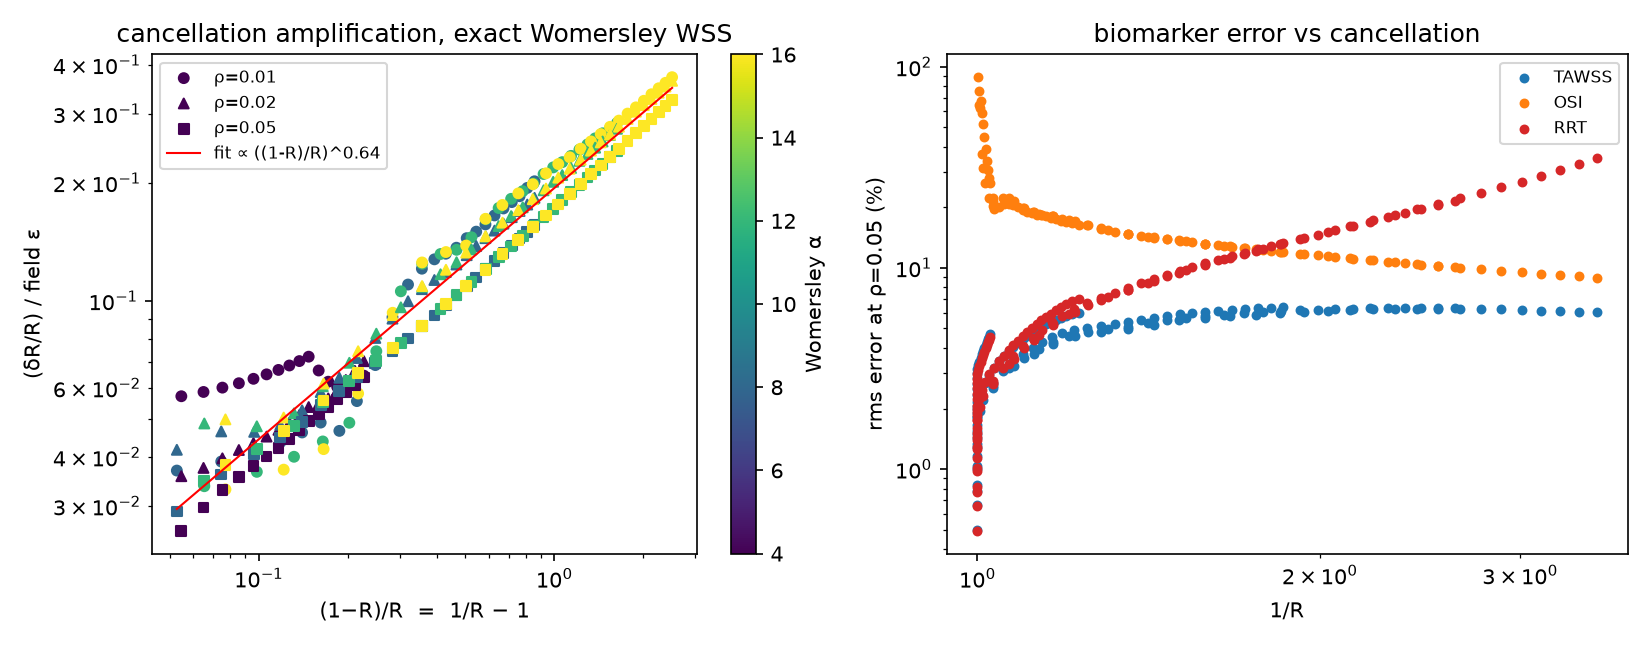
\includegraphics[width=0.85\textwidth]{figs/womersley_sweep.png}
\caption{Womersley sweep. Relative error of the cancellation ratio per unit
field error against the cancellation factor $X=1/R-1$, with the fitted power
law. The fitted exponent $0.64$ is explained in Section~\ref{sec:window} as
the $5/6$--$1$ crossover of \eqref{eq:window} combined with the growth of
$\eps/\rho$ with reversal.}
\label{fig:womersley}
\end{figure}

\subsection{Why $\OSI$ looks fragile in a norm}

From \eqref{eq:chain}, $\delta\OSI/\OSI=-(R/(1-R))\,\delta R/R$, which grows
as $\OSI\to0$: per face, the relative error of $\OSI$ is worst exactly where
$\OSI$ is smallest. In an $L_2$ norm over the wall, however, the faces with
large $\OSI$ dominate the denominator, and on those faces the same expression
is small. The norm-level $\OSI$ error is therefore not a property of $\OSI$
but of the perturbation: white noise inflates it enormously, a window
mismatch barely at all. The often-quoted statement that ``$\OSI$ blows up
because it is small'' is a per-face statement; the large $\OSI$ norm errors
reported in the surrogate literature come from the error type, and
Section~\ref{sec:fingerprint} turns that into a diagnostic.

\section{Injected drift on patient CFD}
\label{sec:cfd}

\paragraph{Cases.}
Two rigid-wall OpenFOAM (v2512) simulations with a physiological inflow
waveform, run to periodicity:
\begin{itemize}
\item a middle-cerebral-artery bifurcation aneurysm (33\,406 wall faces,
$\alpha\approx1.9$, inflow never reverses). Only $0.34\%$ of the wall has
$\OSI>0.1$; the sac maximum is $0.085$. Area-averaged $\TAWSS=\SI{5.73}{Pa}$,
$\OSI=0.0032$. This is the low-reversal control.
\item an abdominal aortic aneurysm (Vascular Model Repository case AAA042,
48\,345 wall faces, 17 cycles to a $2.7\%$ cycle-to-cycle floor). Flow
reversal is physiological here; sac peak $\OSI=0.209$, $2.5\times$ the
cerebral sac. Whole-wall averages are dominated by non-reversing iliac
segments and are not comparable between the two cases; we compare sac to
sac.
\end{itemize}

\paragraph{Protocol.}
The converged last cycle is re-sampled with a clock error $\rho$ (the period
is stretched by $1+\rho$ and the field re-interpolated onto the original time
grid), i.e.\ the window mismatch of Section~\ref{sec:window}: a surrogate
whose limit cycle has the right shape but the wrong, unknown rate, integrated
over the patient's period. Biomarkers are recomputed and compared to the
unperturbed cycle over the whole wall, the sac, and the $\OSI>0.1$ region.
The same wall is also perturbed by a frozen bias and by white noise at
matched field error, to test the exponents of
Sections~\ref{sec:bias} and \ref{sec:window} against each other
(\texttt{law\_vs\_errortype.py}).

\paragraph{Results.}
On the cerebral case at $\rho=5\%$ the raw field $L_2$ is $10.8\%$ while
$\TAWSS/\RRT$ errors are $2.47/2.54\%$ (wall), $3.44/3.57\%$ (sac) and
$1.51/2.42\%$ on the $\OSI>0.1$ faces, i.e.\ $\RRT$ is amplified $1.6\times$
only where cancellation is present, as \eqref{eq:window} predicts. On AAA042
(Figure~\ref{fig:aaa}) the $\RRT$ amplification $(\delta\RRT/\RRT)/
(\delta\TAWSS/\TAWSS)$ against $\OSI$ has a log--log slope of $+0.49$, in
the cancellation-favouring direction; below $\rho\approx3\%$ the residual
periodicity floor masks the injected error and only the trend is trusted.

Table~\ref{tab:etype} compares the three error types on the cerebral wall at
matched field error. The ordering predicted in Section~\ref{sec:theory} is
recovered: a period change integrated over the surrogate's own period costs
nothing; a window mismatch costs $2.4\%$ excess $\RRT$ error in the most
reversing faces, which \eqref{eq:window} predicts as $2.5\%$; a frozen bias
costs $12\%$, five times more, as \eqref{eq:bias1d} requires; and white noise
costs least.

\begin{table}[t]
\centering
\caption{Cerebral wall, matched field error $\eps=10.8\%$. Median per-face
excess $\RRT$ error over $\TAWSS$ error, by cancellation-factor bin
($X=1/R-1$), in \%. Face counts per bin: 31\,233, 1797, 281, 86, 9.}
\label{tab:etype}
\begin{tabular}{l r r r r r}
\toprule
perturbation & $[0,0.02)$ & $[0.02,0.1)$ & $[0.1,0.3)$ & $[0.3,1)$ & $[1,10)$\\
\midrule
period change, own window & 0.00 & 0.00 & 0.00 & 0.00 & 0.00\\
window mismatch, $\rho=5\%$ & 0.06 & 0.13 & 0.05 & 0.92 & 2.37\\
frozen bias & $-0.06$ & 0.17 & 1.11 & 3.51 & 12.08\\
white noise & $-0.63$ & $-0.77$ & $-0.12$ & 0.17 & 1.93\\
\midrule
prediction \eqref{eq:window}, $\eps=10.8\%$ & 0.03 & 0.26 & 0.59 & 1.27 & 2.46\\
\bottomrule
\end{tabular}
\end{table}

\begin{figure}[t]
\centering
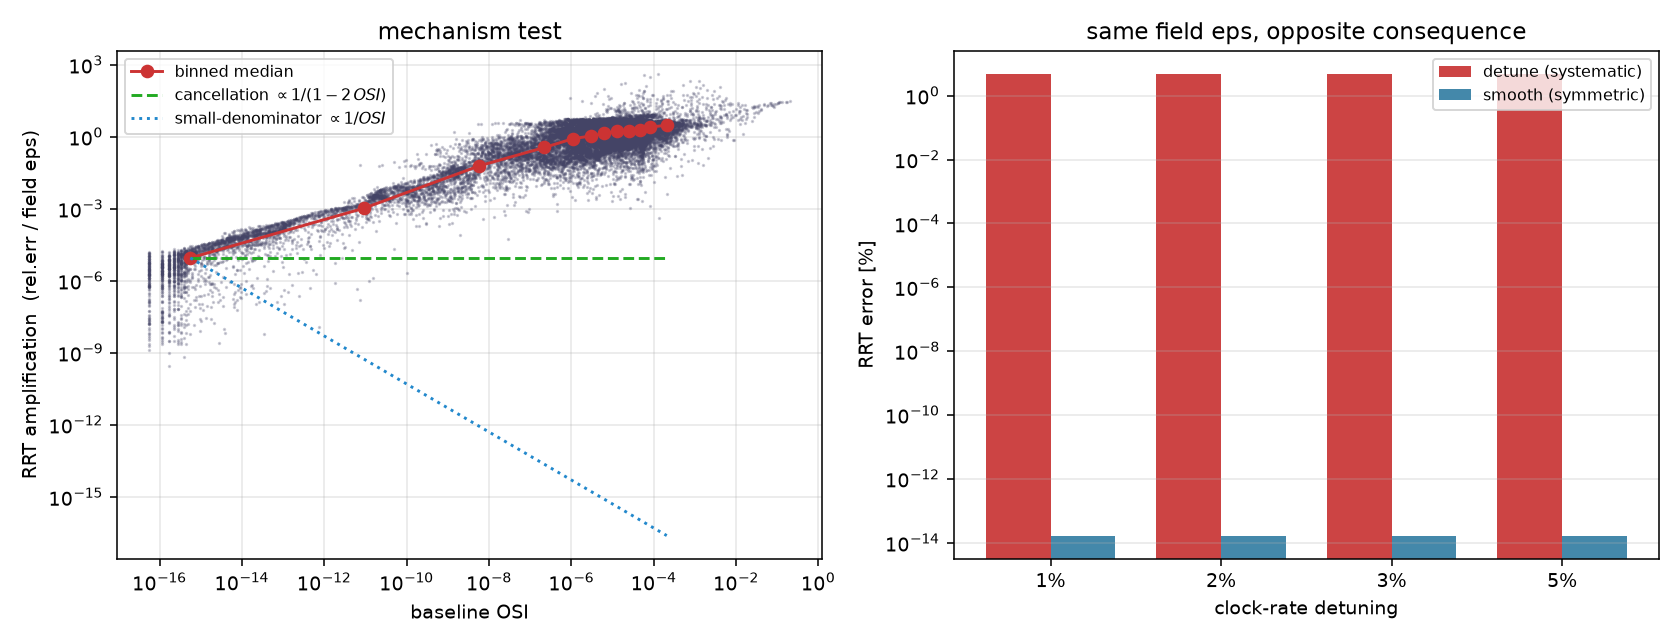
\includegraphics[width=0.85\textwidth]{figs/mechanism_test_aaa042_v2.png}
\caption{AAA042: per-face $\RRT$ amplification versus $\OSI$ under injected
clock drift on the periodic cycle.}
\label{fig:aaa}
\end{figure}

\section{A real surrogate: POD\,+\,LSTM at an unseen heart rate}
\label{sec:lstm}

\paragraph{Model.}
Ten POD modes capture $99.998\%$ of the WSS energy on the cerebral wall; the
compressor alone gives $0.25\%$ field error and $\approx0\%$ $\RRT$ error.
An LSTM is trained on latent trajectories of beats with $34$--$46$ samples
per period (heart-rate augmentation by time stretch, valid at this low
$\alpha$) and tested by autoregressive rollout on the unseen $40$-sample beat
against the CFD truth. A model trained and tested on the same beat memorises
it with zero drift and is kept as the baseline.

\paragraph{What the usual metric says.}
Teacher-forced one-step RMSE on the unseen beat is $7.3\times10^{-2}$ in
latent units, the number a paper would normally report.

\paragraph{What the rollout does.}
Over six beats the raw field $L_2$ grows $7.8\%\to79\%$; after removing the
best global offset it stays at $2$--$10\%$. Lag grows by $\approx0.7$ samples
per beat. A 40-beat rollout is a clean limit cycle with spectral peaks at
$1.013, 2.026, 3.038, 4.051$ per beat: the clock is $1.3\%$ fast, with a weak
$\approx18$-beat wobble (sidebands at $+0.055$ per beat on mode~2). On the
$\OSI>0.1$ faces the $\RRT$ error is $2.3$--$2.7\times$ the $\TAWSS$ error
(Table~\ref{tab:lstm}), consistent with \eqref{eq:chain}.

\begin{table}[t]
\centering
\caption{POD\,+\,LSTM rollout on the unseen beat. Errors in \%. T/R =
$\TAWSS$/$\RRT$.}
\label{tab:lstm}
\begin{tabular}{r r r c c c}
\toprule
beat & raw $L_2$ & lag (samples) & wall T/R & sac T/R & $\OSI>0.1$ T/R\\
\midrule
1 & 7.8 & 0.0 & 6.23/6.78 & 8.84/10.24 & 3.00/6.94\\
2 & 31.2 & $-1.0$ & 7.72/8.59 & 11.59/13.93 & 3.78/9.40\\
3 & 63.1 & $-2.6$ & 2.19/2.30 & 1.99/2.30 & 1.22/1.17\\
4 & 55.6 & $-2.1$ & 9.16/10.40 & 13.36/16.64 & 4.33/11.00\\
5 & 77.3 & $-3.8$ & 1.90/1.88 & 2.62/2.62 & 0.85/1.91\\
6 & 78.9 & $-4.0$ & 1.50/1.56 & 3.54/3.77 & 1.50/4.11\\
\bottomrule
\end{tabular}
\end{table}

\paragraph{Truth-free clock diagnosis.}
Treating the rollout as a limit cycle, the rate error is estimated from the
rollout alone by fitting a single frequency scaling to its own phase
(a phase-reduction view in the sense of Taira and Nakao; the method is that
of~\cite{samanta2026} for bluff-body wakes). On six beats it returns $+1.66\%$
against a ground-truth lag growth of $+1.98\%$; on 40 beats $+1.41\%$, in
agreement with the spectral estimate; after re-timing the residual self-rate is
$-0.03\%$ and the lag stays bounded in $[-2.6,0]$ samples over 40 beats
(Figure~\ref{fig:phase})
(the raw lag reached $-20$ and wrapped). On a synthetic rollout with a known
$2\%$ drift the estimate is $1.99\%$ and re-timing cuts $\RRT$ error
$30\times$.

\paragraph{Re-timing does not repair the biomarkers.}
On the real rollout, mean $\RRT$ error after the transient moves from
$4.95\to4.54\%$ (wall), $7.85\to7.09\%$ (sac), $5.52\to5.10\%$ ($\OSI>0.1$).
A perfect-shape model with a $1.5\%$ clock error would give only
$\approx0.8\%$ $\RRT$ error, so roughly $80\%$ of the error is beat shape and
the slow wobble; $\RRT$ error tracks the offset-removed $L_2$, not the lag.
The check has therefore done its job: it decomposes the error and says
``re-timing will not help; improve the model''. The residual is also
quantitatively consistent with the theory. Applying the window-mismatch
formula \eqref{eq:window} with the offset-removed $\eps=3.7\%$ predicts an
excess $\RRT$ error of $0.8\%$ in the top cancellation bin
($X\in[1,10)$), while the measured excess is $7.0\%$ --- a factor of nine
too small. But after re-timing the residual is by construction \emph{not} a
window mismatch: it is beat-shape error, which is persistent across the
rollout and therefore closer to the bias case of Section~\ref{sec:bias},
whose prefactor is about five times larger and whose exponent is $1$ rather
than $0.76$. The under-prediction is thus the expected signature of applying
the wrong error model, and is itself part of the diagnosis.

\begin{figure}[t]
\centering
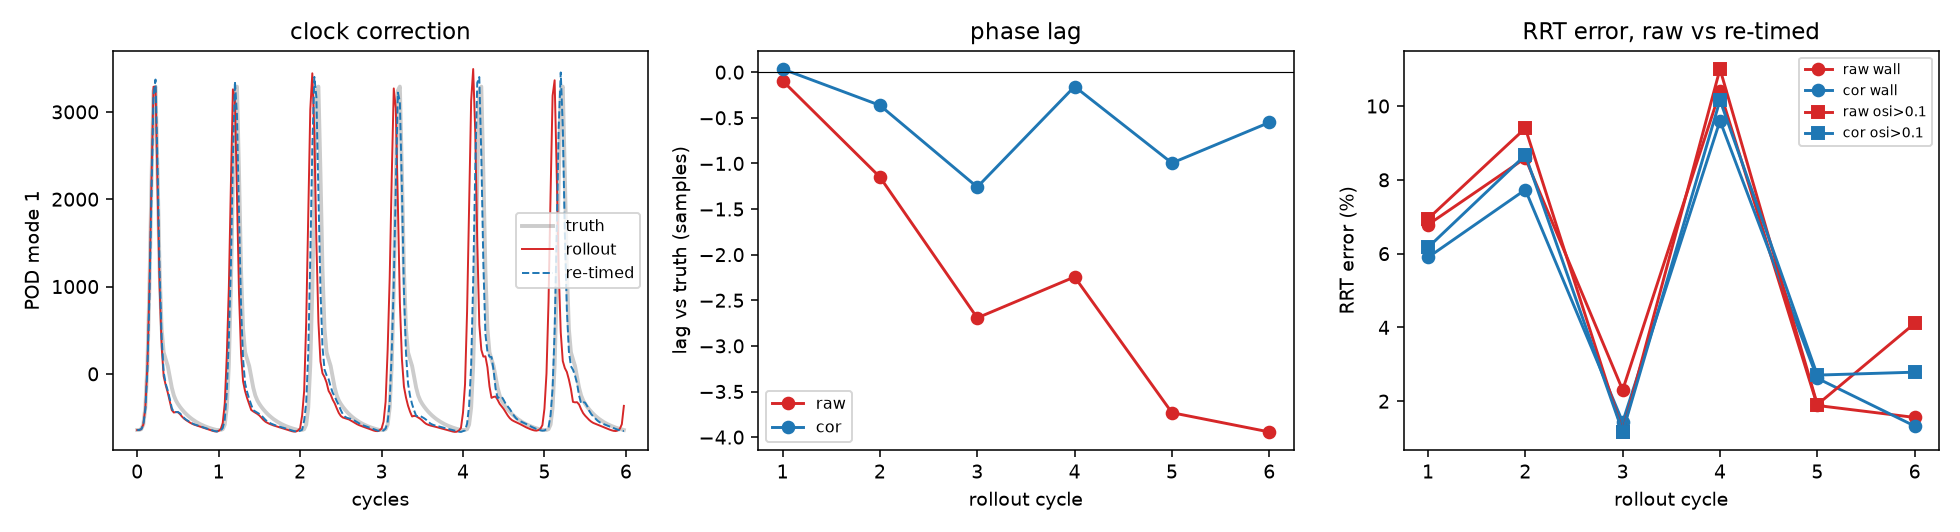
\includegraphics[width=0.85\textwidth]{figs/phase_correct_hr.png}
\caption{Truth-free clock estimate and re-timing on the six-beat rollout.}
\label{fig:phase}
\end{figure}

\section{The error triple as a fingerprint, and an external check}
\label{sec:fingerprint}

The cerebral cycle was perturbed in four ways at matched field error
$\eps$ and the biomarkers were scored with the mean-based relative $L_2$
used by RHSIA~\cite{rhsia2026}, $\|X_{\rm pred}-X_{\rm true}\|_2/\|X_{\rm true}\|_2$
over faces: (i)~clock drift; (ii)~Gaussian noise independent per face and per
snapshot (\emph{white}); (iii)~Gaussian noise per face, constant in time
(\emph{frozen} bias); (iv)~the window-mismatch prediction \eqref{eq:window}
applied face by face.
Table~\ref{tab:fp} lists the results next to RHSIA's published Table~V,
obtained on a per-snapshot graph model over intracranial aneurysm surfaces.

\begin{table}[t]
\centering
\caption{Biomarker error ratios by error type on the cerebral wall,
mean-based $rL_2$ in \%, versus RHSIA~\cite{rhsia2026} Table~V.}
\label{tab:fp}
\begin{tabular}{l r r r r r r}
\toprule
perturbation & $\eps$ & $\TAWSS$ & $\OSI$ & $\RRT$ & $\OSI/\TAWSS$ & $\RRT/\TAWSS$\\
\midrule
prediction \eqref{eq:window}, per face & 13.5 & 13.5 & 5.1 & 13.6 & 0.37 & 1.00\\
clock drift $\rho=5\%$ & 10.8 & 2.5 & 3.1 & 3.5 & 1.22 & 1.37\\
white noise & 13.5 & 2.3 & 68.7 & 2.5 & 30 & 1.08\\
frozen bias & 13.5--16 & 10--12 & 57--75 & 14--19 & 5.6--6.3 & 1.4--1.6\\
\midrule
RHSIA (published) & -- & 13.54 & 68.35 & 17.31 & 5.05 & 1.28\\
\bottomrule
\end{tabular}
\end{table}

Two things follow. First, $\RRT/\TAWSS\approx1.3$ is obtained for every
error type on a low-reversal wall and matches RHSIA's $1.28$: on such a wall
\eqref{eq:chain} reduces to $\delta\RRT\approx\delta\TAWSS$ plus a small
cancellation term, and an independent model confirms it. Second,
$\OSI/\TAWSS$ separates the error types by more than an order of magnitude,
and only a time-coherent per-node bias reproduces RHSIA's $5.05$. That is
the error one expects from a model that regresses each snapshot
independently from geometry: its mistakes are spatial and persistent, not
temporal, exactly the case of Section~\ref{sec:bias}. The window-mismatch
formula predicts $0.37$ and is simply the wrong error model for that
surrogate --- which the fingerprint detects without needing to be told.
The corresponding author of RHSIA confirms the reading: ``you were right
about the RRT error of my surrogate model, they present spatial error and
usually persistent''. The three numbers every surrogate
paper already reports therefore say which remedy applies: a ratio near~1
with a drifting lag calls for re-timing; a very large ratio with small
$\TAWSS$ error indicates temporal noise that smoothing removes without
touching $\RRT$; an intermediate ratio with comparable $\TAWSS$ and $\RRT$
errors indicates spatial bias that only a better model repairs.

The cerebral $\OSI$ distribution (median $7\times10^{-4}$, $94\%$ of faces
below $0.01$) is used here as a proxy for RHSIA's surfaces; the
frozen-bias numbers vary by $\pm15\%$ with the random seed.

\section{Discussion and limitations}

\begin{itemize}
\item The master relation \eqref{eq:master} is elementary; its value is in
the consequences, which are routinely violated in practice: scoring a rollout
by raw $L_2$, reading a large $\OSI$ error as a property of $\OSI$ rather
than of the perturbation, reporting one-step accuracy for a model whose limit
cycle runs at the wrong rate, and applying one error model's constants to a
different error type.
\item The closed forms are first order in $|\mathbf d|/|\boldsymbol\tau|$ and
assume the perturbation does not itself change the sign structure of the
waveform. At $X\lesssim0.02$ the bias formula is only accurate to a factor of
two, and the discrete window-mismatch experiment departs from
\eqref{eq:window} by up to $58\%$ at the smallest $X$, where a $1\%$ slice of
a 40-sample cycle is sub-sampled.
\item The $5/6$ exponent holds at the onset of reversal for smooth
waveforms. Real surrogate errors mix the three types, and the mixture is not
derived here --- the fingerprint identifies the dominant one, not the
decomposition.
\item Evidence rests on two geometries, one of which has very little
reversal, and on a single small surrogate. The external check uses
published aggregate numbers, not RHSIA's fields.
\item Entrainment of the surrogate to an external clock (Arnold-tongue
picture), a graph-network surrogate on the same data, and a systematic
literature audit of which surrogate papers report $\OSI/\RRT$ and check for
drift are future work.
\end{itemize}

\section*{Data and code availability}
All scripts (\texttt{womersley\_sweep.py}, \texttt{law\_theory.py},
\texttt{law\_theory\_bias.py}, \texttt{law\_vs\_errortype.py},
\texttt{pod\_lstm\_hr\_v2.py}, \texttt{phase\_correct\_v2.py},
\texttt{mechanism\_test\_aaa042\_v2.py}, \texttt{rhsia\_check\_v[1-3].py})
and the reduced data needed to reproduce the figures are at
\url{https://github.com/Syphonicc/shear-drift}, with the interactive version
at \url{https://syphonicc.github.io/shear-drift/}. AAA042 is from the Vascular
Model Repository. OpenFOAM runs used CloudHPC.

\section*{Acknowledgements}
This work was carried out for the UnivaXBio hackathon (Devpost, October
2026), where it is packaged as an interactive surrogate ``unit test''.
The author thanks Sachidananda Behera for discussions, and Wenhao Ding
(Imperial College London) for the observation that a period change integrated
over the surrogate's own cycle is harmless, which corrected
Section~\ref{sec:window}.

\begin{thebibliography}{9}
\bibitem{npj2026} Physics-constrained graph neural network for real-time
prediction of intracranial aneurysm hemodynamics. \emph{npj Digital Medicine}
(2026). \url{https://doi.org/10.1038/s41746-026-02404-z}
\bibitem{jekenrico2025} Graph deep learning for intracranial aneurysm blood
flow simulation and risk assessment. arXiv:2512.09013 (2025).
\bibitem{rhsia2026} Real-time pulsatile flow prediction for realistic,
diverse intracranial aneurysm morphologies using a graph transformer and
steady-flow data augmentation (RHSIA). arXiv:2601.19876v2 (2026).
\bibitem{rygiel2025} Rapid wall shear stress prediction for aortic aneurysms
using deep learning. \emph{Med.\ Biol.\ Eng.\ Comput.} (2025).
\url{https://doi.org/10.1007/s11517-025-03311-3}
\bibitem{aaa2025} Wall shear stress estimation in abdominal aortic aneurysms:
towards generalisable neural surrogate models. arXiv:2507.22817 (2025).
\bibitem{sarrami2016} Sarrami-Foroushani A.\ et al. Uncertainty
quantification of wall shear stress in intracranial aneurysms using a
data-driven statistical model of systemic blood flow variability.
\emph{J.\ Biomech.} 49 (2016).
\bibitem{bergersen2017} Bergersen A.\ W.\ et al. Robustness of common
hemodynamic indicators with respect to numerical resolution in 38 middle
cerebral artery aneurysms. \emph{PLoS ONE} 12 (2017) e0177566.
\bibitem{mri2016} The effect of spatial and temporal resolution of cine
phase-contrast MRI on wall shear stress and oscillatory shear index
assessment. \emph{PLoS ONE} (2016). PMID 27669568.
\bibitem{samanta2026} Samanta S., Behera S. Autoregressive rollout error in
latent-space reduced-order models of bluff-body wakes is accumulated phase
drift. arXiv:2608.07189 (2026).
\end{thebibliography}

\end{document}
